\clearpage
\twocolumn[{%
\rqparent
\subsection{Subset selection}
\label{app:rq08_subset_selection}

\noindent\begin{minipage}[t]{0.485\textwidth}
\vspace{0pt}
\paragraph{Research Question.} \emph{For each benchmark, does a subset of its subtasks (the \emph{languages} of a multilingual family, the \emph{subjects} of MMLU or single \emph{items}) give a higher SNR than the full set, and does the same subset hold across seeds and scales?}

\paragraph{Setup.} We test whether the best subset of a benchmark's languages separates the designs better than a random subset of the same size, comparing the SNR of the two. We use the seed-1904 runs of every cell, ladder and data build, 90M--1.7B. The tasks are the per-language tasks of each multilingual benchmark that pass the above-chance gate at each size, plus their bBPB versions. We rank the languages by their own SNR and score each prefix of that ranking (the top language, the top two, and so on). The prefix with the highest SNR is the chosen subset, and we compare it with the 95th percentile of 100 random subsets of the same size.
\end{minipage}\hfill
\begin{minipage}[t]{0.485\textwidth}
\vspace{0pt}
\begin{rqfinding}
\textbf{1. A chosen language subset beats the random-subset null in a minority of cases.} It does so in 94 of the 254 swept Case-1 (benchmark, size) cells, which are 94 of the 221 Case-1 cells with a positive raw gain. The highlighted result above counts every case, so it reads 100 of 227 (the six Case 2 and 3 cells all beat their null). In Case 1 the subset beats the null by more than 0.25 SNR in 66 cells. HellaSwag (median +1.12 over six sizes), ARC (+0.97 over four), MultiBLiMP (+0.65) and Global-MMLU RF (+0.61) gain the most. XStoryCloze, LAMBADA, XWinograd and the BPB family never beat the null, XCOPA beats it only once (+0.02), and PAWS-X sits below it (median $-$0.13). (Figure~\ref{fig:app_rq08_subset_selection}.)
\\
\\
\textbf{2. Without the null, a subset seems to help almost everywhere.} The best prefix beats the full set in 221 of the 254 Case-1 cells that have an SNR (median +0.80 SNR), but only 94 of these 221 cells also beat the null.
\\
\\
\textbf{3. Accuracy families and bBPB twins beat the null about equally often.} In the accuracy and BPB families 67 of 151 cells beat the null (33 benchmarks), against 27 of 70 for the bBPB twins (14 twins, read on their full noise window).
\end{rqfinding}
\end{minipage}
\vspace{\baselineskip}
}]

\begin{figure*}[p]
\centering
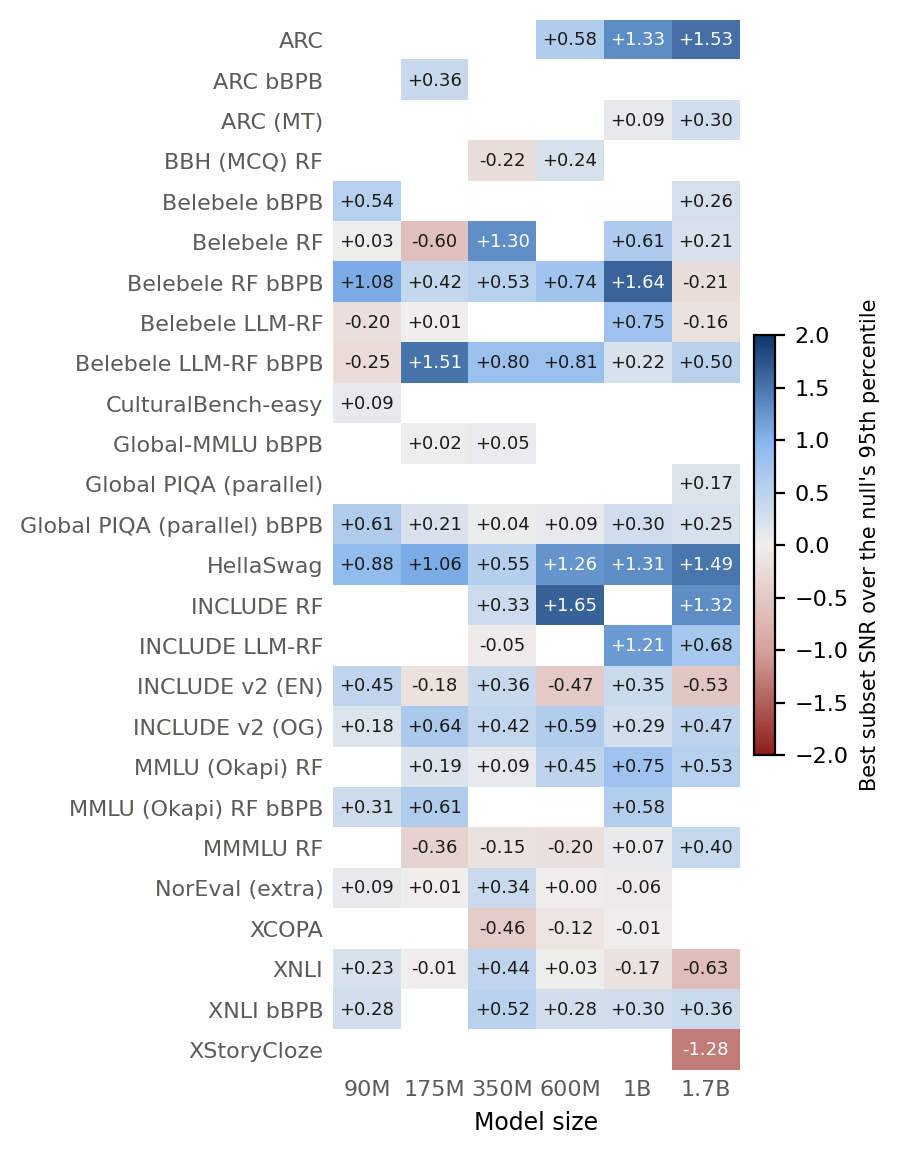
\includegraphics[width=0.8\textwidth,height=0.8\textheight,keepaspectratio]{figures/app_rq08_subset_selection.png}
% source: src/signal-and-noise/analysis/rq08_subset_selection/pretraining/predictivity/gain_over_null_paper.png
\caption{\textbf{A chosen language subset beats the random-subset null in a minority of cells.} For each benchmark (rows, accuracy and bBPB versions) and model size (columns), the SNR of the best language subset minus the 95th percentile of 100 random subsets of the same size. Blue means that the chosen subset beats the null. White cells have no value.}
\label{fig:app_rq08_subset_selection}
\end{figure*}
